%++++++++++++++++++++++++++++++++++++++++
% Don't modify this section unless you know what you're doing!
\documentclass[letterpaper,12pt]{article}
\usepackage{tabularx} % extra features for tabular environment
\usepackage{amsmath}  % improve math presentation
\usepackage{graphicx} % takes care of graphic including machinery
\usepackage[margin=1in,letterpaper]{geometry} % decreases margins
\usepackage{cite} % takes care of citations
\usepackage[final]{hyperref} % adds hyper links inside the generated pdf file
\hypersetup{
	colorlinks=true,       % false: boxed links; true: colored links
	linkcolor=blue,        % color of internal links
	citecolor=blue,        % color of links to bibliography
	filecolor=magenta,     % color of file links
	urlcolor=blue         
}
%++++++++++++++++++++++++++++++++++++++++


\begin{document}

\title{SMART COFFEE VENDING MACHINE }
\author{Nakshatiraa Natarjan - 211101080}

\maketitle



\section{ABSTRACT}

This paper describes how to utilize the Internet of Things (IoT) concept for upgrading a franchisor’s traditional coffee vending machine to be a smart coffee vending machine (SCVM) with remote monitoring and control capabilities. The IoT-based SCVM provides powerful web dashboard to monitor machine operation statuses, track ingredient and component availability, and adjust hot drink recipes.


 

	This system provides ideal solution to the problems faced by home owners in daily life. In addition the application was a need to automate valve of coffee maker so that user can take advantage of the technological advancement in such a way that a person getting off the office and ready to serve the coffee. This type of remote control capability and possibility of achieving at a reasonably low cost.



\section{WORKING PRINCIPLE}

The process of controlling a valve will proceed through the following: Assume that the equipments are fed with electric current and operating properly. Initially the user sends the command through the SMS from mobile phone to GSM modem. GSM modem is connected to Arduino microcontroller via RS232 serial port connection. The MAX232 Driver can be used to convert the TTL logic into RS232 level logic. Microcontroller keeps polling to check if the
modem has received any text message. When the GSM receiver receives the message it will sends to microcontroller. GSM modem and arduino microcontroller can communicate through AT COMMANDS. It is a special type of command. It is an abbreviation of Attention Command. Microcontroller sends another command to the GSM modem to delete the current SMS for process the next SMS. Finally microcontroller analyzes the command and instructs the relay to switch ON/OFF.




\section{SYSTEM ARCHITECTURE}

                    In this system the main components are GSM modem and arduino microcontroller both are IoT devices. A text message is sent by the user through the GSM network. The GSM receiver which receives the messages and sends to the arduino microcontroller. All the devices are connected to the central control system of arduino microcontroller. The MAX232 is an integrated circuit which can be used to convert the TTL logic level to RS232 logic level. The microcontroller analyzes the command and instructs the relay. Based on that relay operates the solenoid valve



\section{PROTOCOL}

The process of controlling a valve will proceed through the following: Assume that the equipments are fed with electric current and operating properly. Initially the user sends the command through the SMS from mobile phone to GSM modem. GSM modem is connected to Arduino microcontroller via RS232 serial port connection. The MAX232 Driver can be used to convert the TTL logic into RS232 level logic. Because of GSM and microcontroller which only understood the machine language. Microcontroller keeps polling to check if the modem has received any text message. When the GSM receiver receives the message it will sends to microcontroller. GSM modem and arduino microcontroller can communicate through AT COMMANDS. It is a special type of command. It is an abbreviation of Attention Command. Microcontroller sends another command to the GSM modem to delete the current SMS for process the next SMS. Finally microcontroller analyzes the command and instructs the relay to switch ON/OFF. According to that relay operates the solenoid valve.

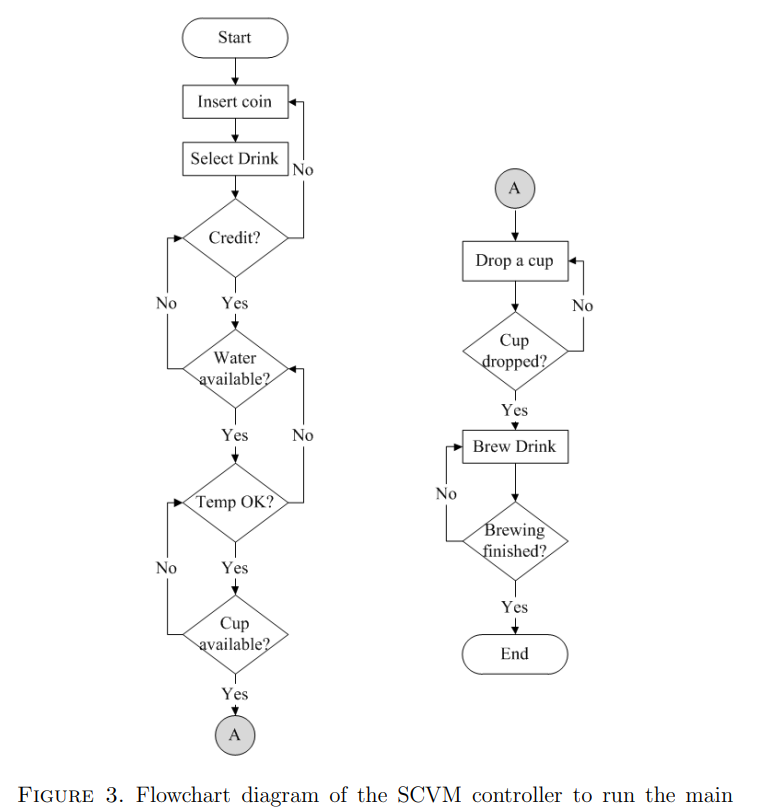
\includegraphics[scale=0.6]{cup.png}

The franchisor and franchisees can access the technical and sales data via the created web dashboard by employing user login system.In order to ensure that hot drinks are always available to offer customers, the franchisor can monitor the real-time operation statuses of all SCVMs, which are connected into the cloud computing service.

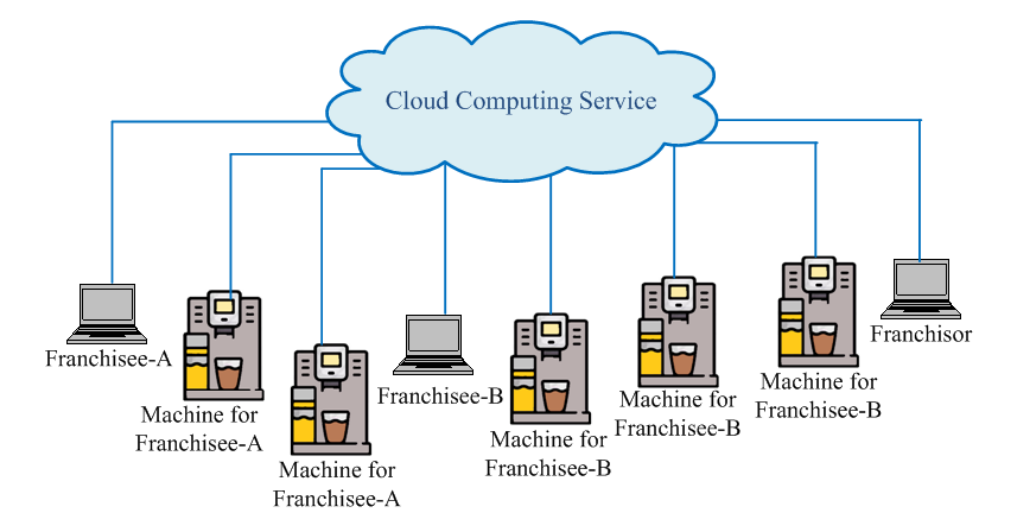
\includegraphics[scale=0.5]{cloud.png}

In addition, the ingredient and component availability and the drink recipes of each SCVM can be tracked and adjusted, respectively. However, the franchisee is allowed to monitor the operation status and daily sales data for his approved machines only.

\section{ADVANTAGES}

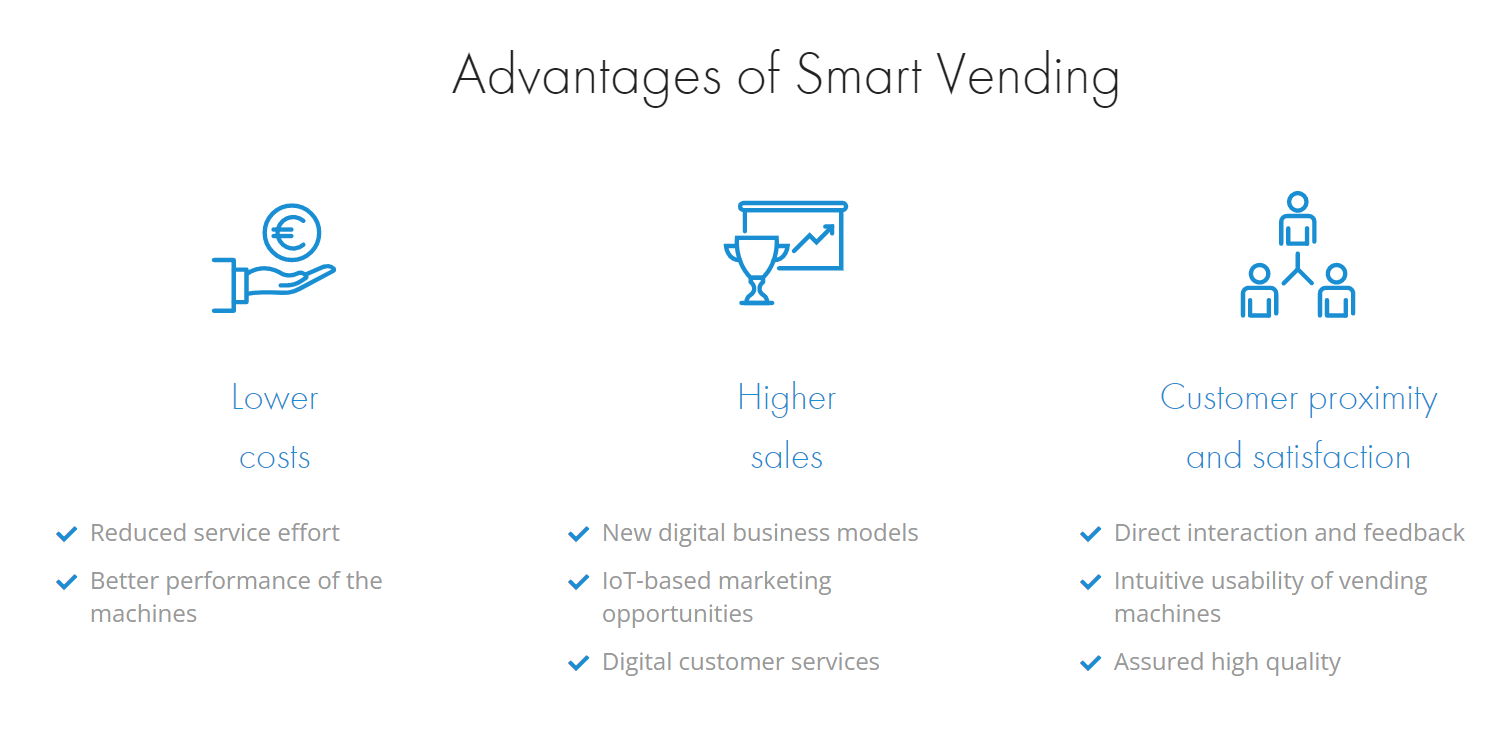
\includegraphics[scale=0.4]{adv.png}



\section{CONCLUSIONS}
The implementation of IoT based coffee vending machine helps the customer to order the coffee according to their taste
via a mobile app. They just need to select the type thy want and just click on order coffee. The level of ingredients is
continuously monitored and before they get emptied in the machine. The notification alert is send to the concerned
department to fill the required ingredient. It aims at advanced management of the whole coffee vending machine
previously used

\section{References}
[1] K. Kim, D-H. Park, H. Bang, G. Hong and S-I. Jin, Smart coffee vending machine using sensor and
actuator networks, Proc. of 2014 IEEE Conference on Consumer Electronics, Las Vegas, NV, USA,
pp.71-72, 2014.


[2] Y. Ishii, E. Saneyoshi, M. Sendoda and R. Kondo, Anomaly identification in a liquid-coffee vending
machine using electrical current waveforms, Proc. of IEEE the 2nd Conference on Information and
Computer Technologies, Kahului, HI, USA, pp.98-101, 2019.


[3] C. Wanmahajai, T. Thepmanee and S. Pongswatd, Integration of WirelessHART into SCADA system
and information applications, ICIC Express Letters, vol.10, no.1, pp.95-101, 2016.


[4] A. Tanyakorn, S. Pongswatd, A. Julsereewong and A. Rerkratn, Integration of WirelessHART and
ISA100.11a field devices into condition monitoring system for starting IIoT implementation, Proc. of
the 56th Annual Conference of the Society of Instrument and Control Engineers of Japan, Kanazawa,
Japan, pp.1395-1400, 2017.


\end{document}
